\section{Experimentos e resultados} 

Para poder fazer cada experimento foi utilizado o programa toysat \cite{ToySAT14} e um script para ter varios threads em paralelo tão para gerar os datos como para executar toysat solver.

\subsection{Experimento 1}
	\subsubsection{Descrição}
		Para $K = 3$ (ou seja, 3-SAT) e $N = 100$, levantar a curva de resposta de tempo, e apresentá-la sobreposta à curva de percentagem de problemas satisfazíveis. Cada ponto deve ser obtido a partir de pelo menos 100 instâncias geradas aleatoriamente. Apresentar e discutir o formato do gráfico.
	\subsubsection{Resultados}
		\begin{figure}[H]
			\centering
			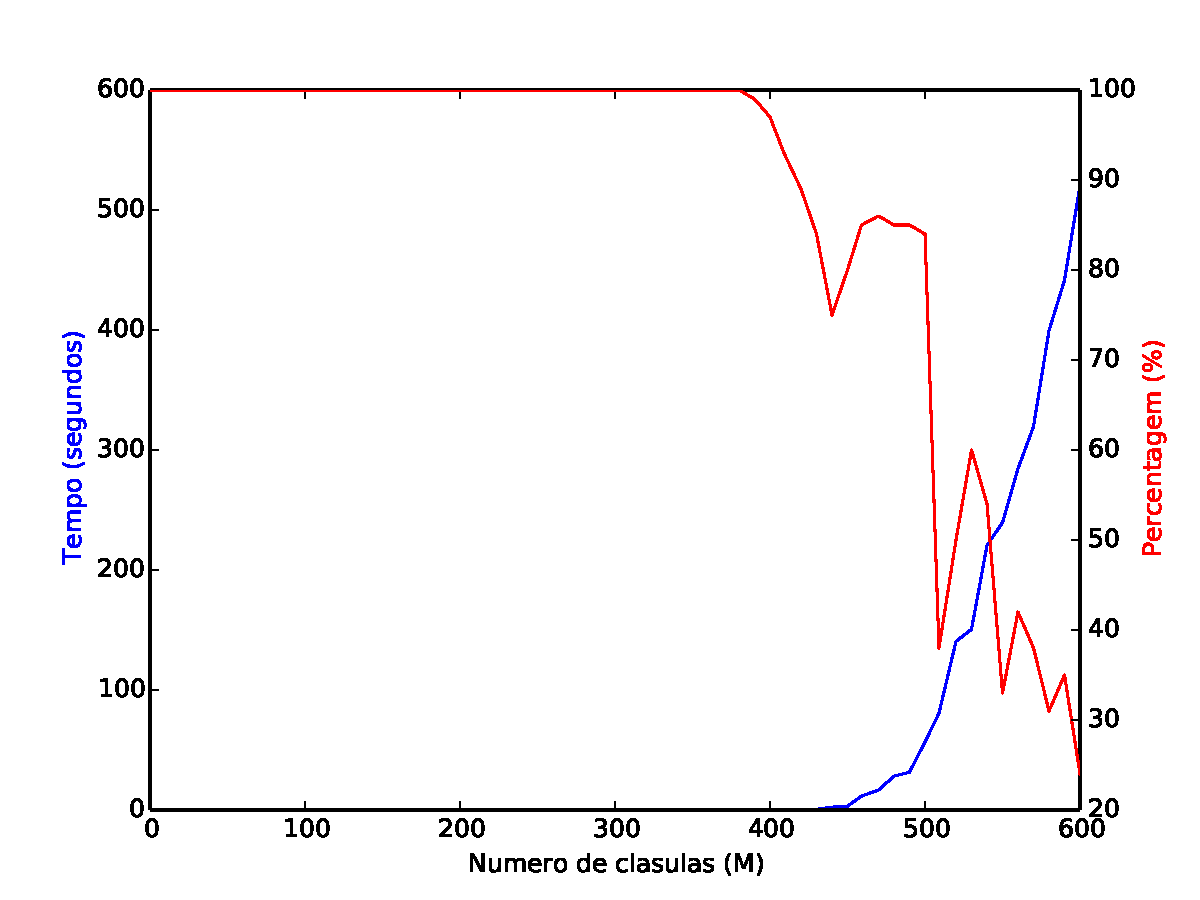
\includegraphics[height=10cm]{images/max3sat_100at}
			\caption{Curva de resposta de tempo (azul), curva de percentagem (vermelho)}
			\label{fig:max3sat100at}
		\end{figure}
	
 \subsection{Experimento 2}
	\subsubsection{Descrição}
		Para $K = 2$ (ou seja, 2-SAT) e $N = 100$, levantar a curva de resposta de tempo, e apresentá-la sobreposta à curva de percentagem de problemas satisfazíveis. Cada ponto deve ser obtido a partir de pelo menos 100 instâncias geradas aleatoriamente. Apresentar e discutir o formato do gráfico.
	\subsubsection{Resultados}
		\begin{figure}[H]
			\centering
			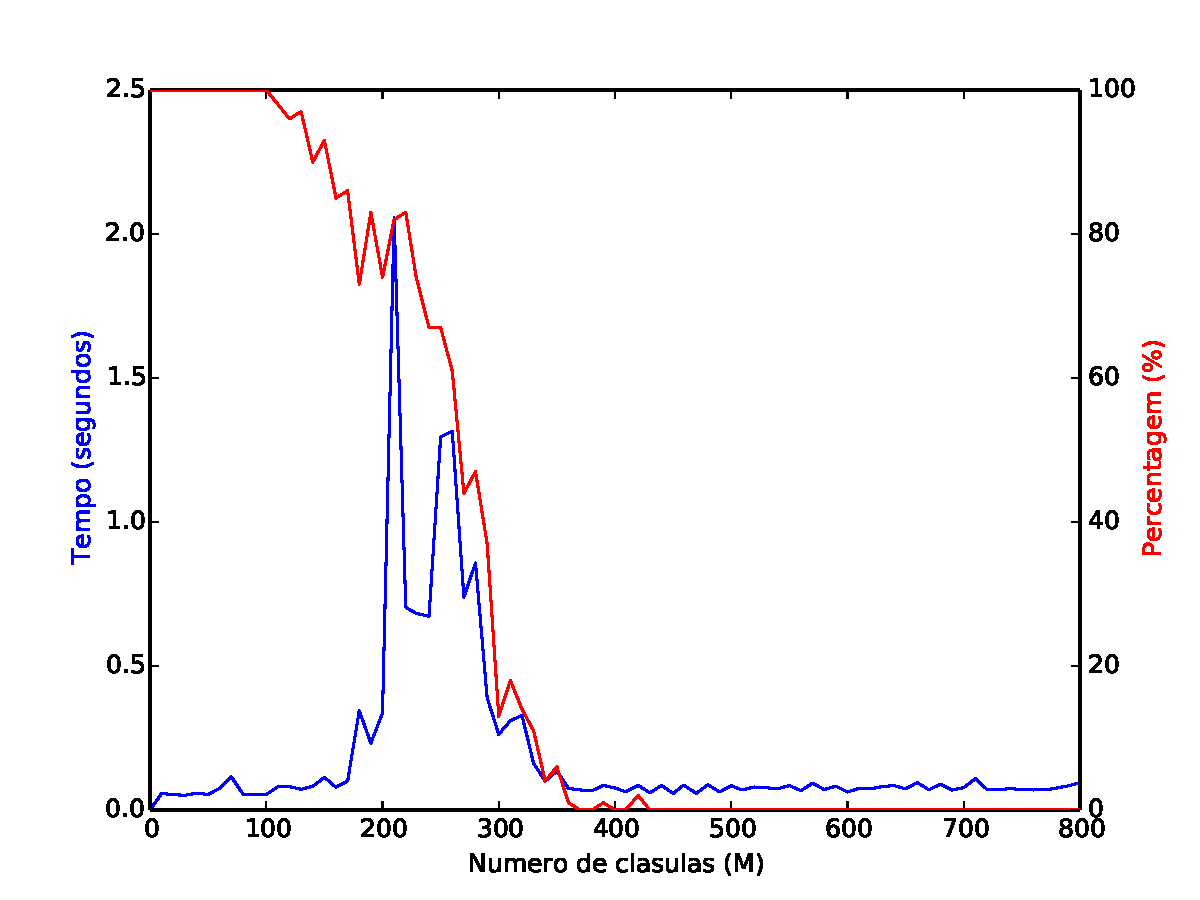
\includegraphics[height=10cm]{images/max2sat_100at}
			\caption{Curva de resposta de tempo (azul), curva de percentagem (vermelho)}
			\label{fig:max2sat100at}
		\end{figure}

\subsection{Experimento 3}
	\subsubsection{Descrição}
		Apresentar 5 gráficos mostrando o tempo de execução em função de $N$ para $K = 3$. Em cada gráfico, o valor de $M / N$ deve ser fixo. Os cinco gráficos devem ser feitos para $N$ variando de 100 a 1000, em intervalos de 100. Os valores de $M / N$ de cada um dos 5 gráficos são 1; 3; 4,3; 6; e 8. Discutir a natureza da curva obtida em cada caso, se polinomial ou exponencial.
	\subsubsection{Resultados}
		\begin{table}[!htb]
			\centering{
				\resizebox{.9\columnwidth}{!}{
					\begin{tabular}{|c|r|r|r|r|r|} \hline
						\multicolumn{1}{|c|}{{N}} & \multicolumn{1}{|c|}{{$M/N=1.0$}} & \multicolumn{1}{|c|}{{$M/N=3.0$}} & \multicolumn{1}{|c|}{{$M/N=4.3$}} & \multicolumn{1}{|c|}{{$M/N=6.0$}} & \multicolumn{1}{|c|}{{$M/N=8.0$}} \\ \cline{1-6}
						100    & 0.042 & 0.050 & 10.278  & 6327.574 & 100.724 \\\hline
						200    & 0.092 & 0.137 & 58.735  & 7732.361 & 224.791 \\\hline
						300    & 0.071 & 0.108 & 116.031 & 15253.935 & 384.112 \\\hline
						400    & 0.131 & 0.322 & 230.58 & 40823.234 & 681.084 \\\hline
						500    & 0.178 & 0.434 & 512.05 & 91834.454 & 800.268 \\\hline
						600    & 0.196 & 0.422 & 741.912 & 131082.805 & 811.481 \\\hline
						700    & 0.168 & 0.668 & 998.048 & - & 811.101 \\\hline
						800    & 0.188 & 0.763 & 1806.502 & -  & 842.849 \\\hline
						900    & 0.296 & 0.765 & 2501.011 & -  & 895.298 \\\hline
						1000  & 0.199 & 0.717 & 4700.17 & - & 874.026 \\\hline
					\end{tabular}
        				}
			}
			\label{tab:3satTempos}
			\caption{Comparação de tempos (segundos) de Max 3-SAT}
		\end{table}
		
		\begin{figure}[H]
			\centering
			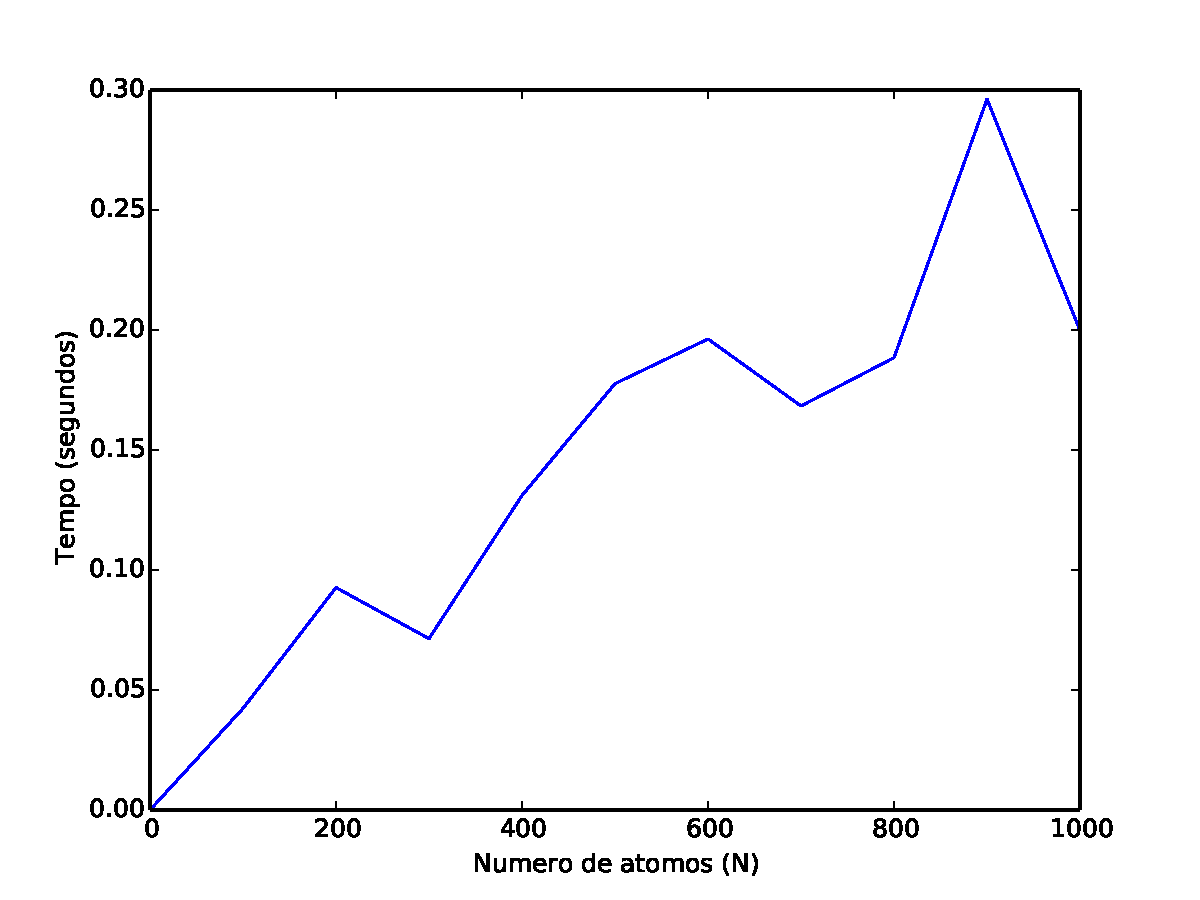
\includegraphics[height=10cm]{images/max3sat_mn10}
			\caption{Curva de resposta de tempo para $M/N=1.0$}
			\label{fig:max3satmn10}
		\end{figure}
		
		\begin{figure}[H]
			\centering
			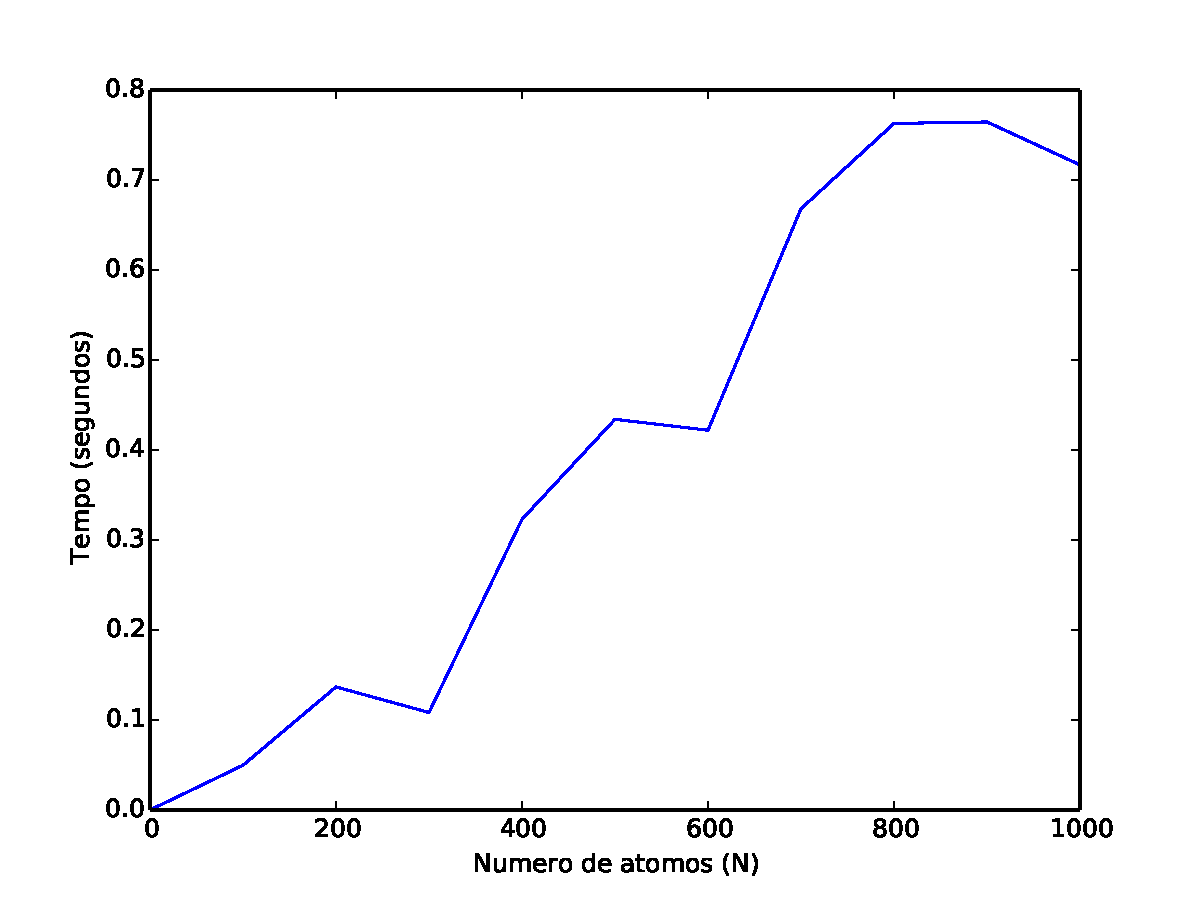
\includegraphics[height=10cm]{images/max3sat_mn30}
			\caption{Curva de resposta de tempo para $M/N=3.0$}
			\label{fig:max3satmn30}
		\end{figure}
		
		\begin{figure}[H]
			\centering
			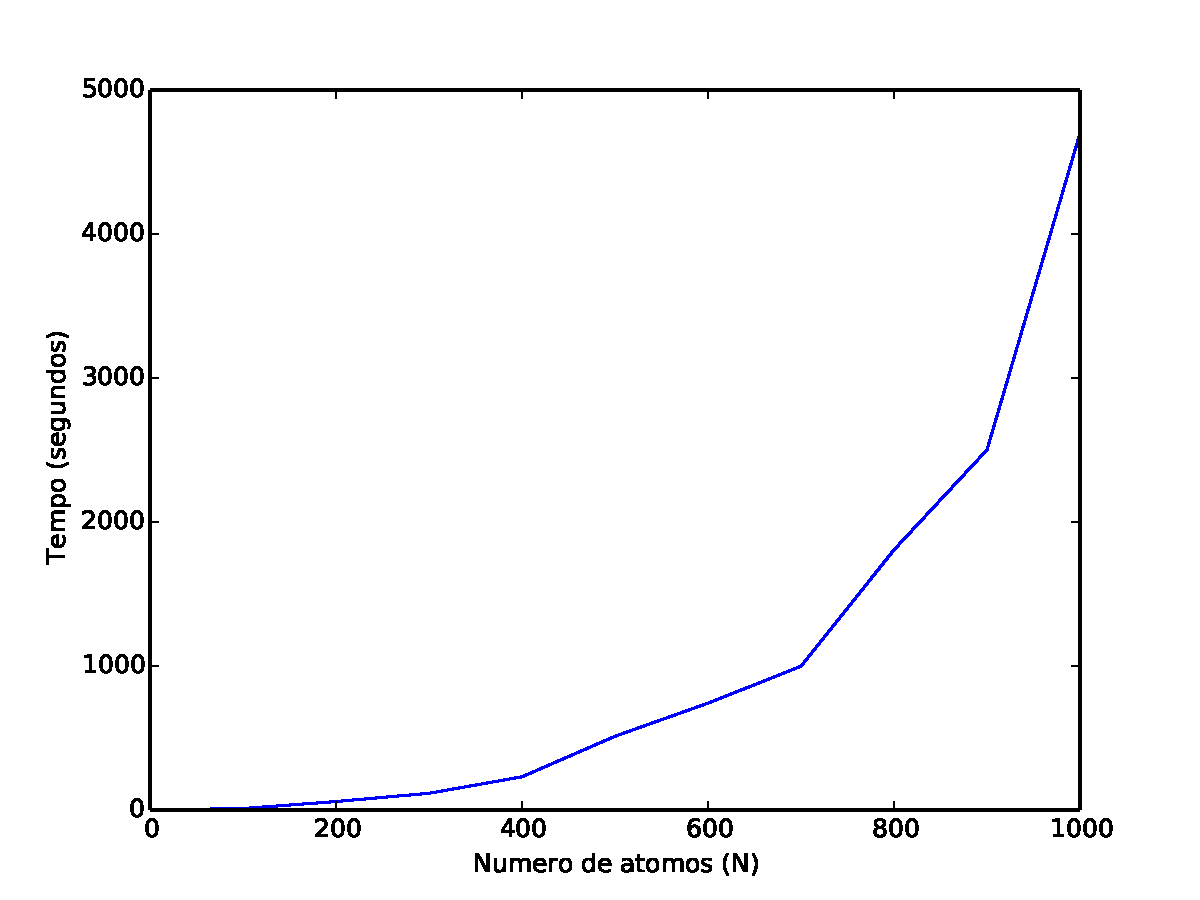
\includegraphics[height=10cm]{images/max3sat_mn43}
			\caption{Curva de resposta de tempo para $M/N=4.3$}
			\label{fig:max3satmn43}
		\end{figure}
		
		\begin{figure}[H]
			\centering
			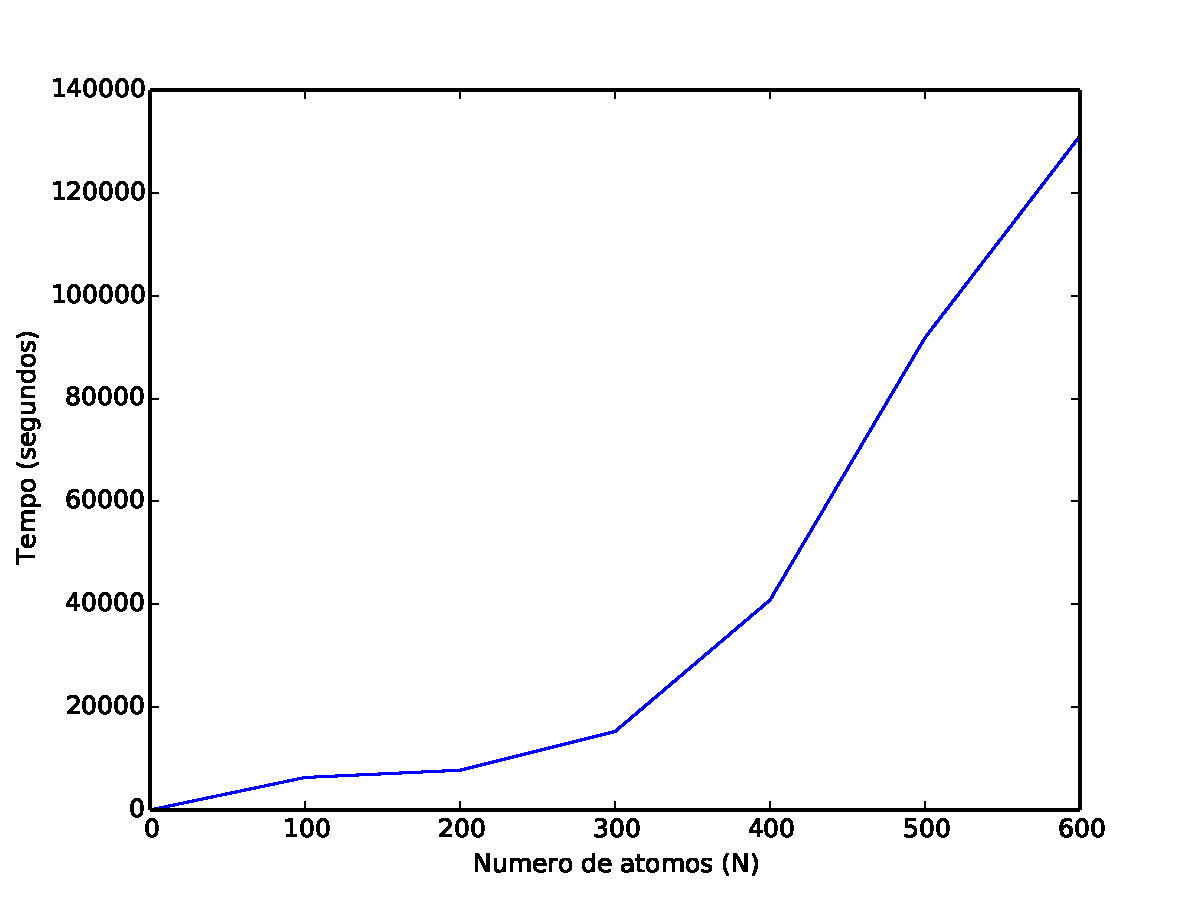
\includegraphics[height=10cm]{images/max3sat_mn60}
			\caption{Curva de resposta de tempo para $M/N=6.0$}
			\label{fig:max3satmn60}
		\end{figure}
		
		\begin{figure}[H]
			\centering
			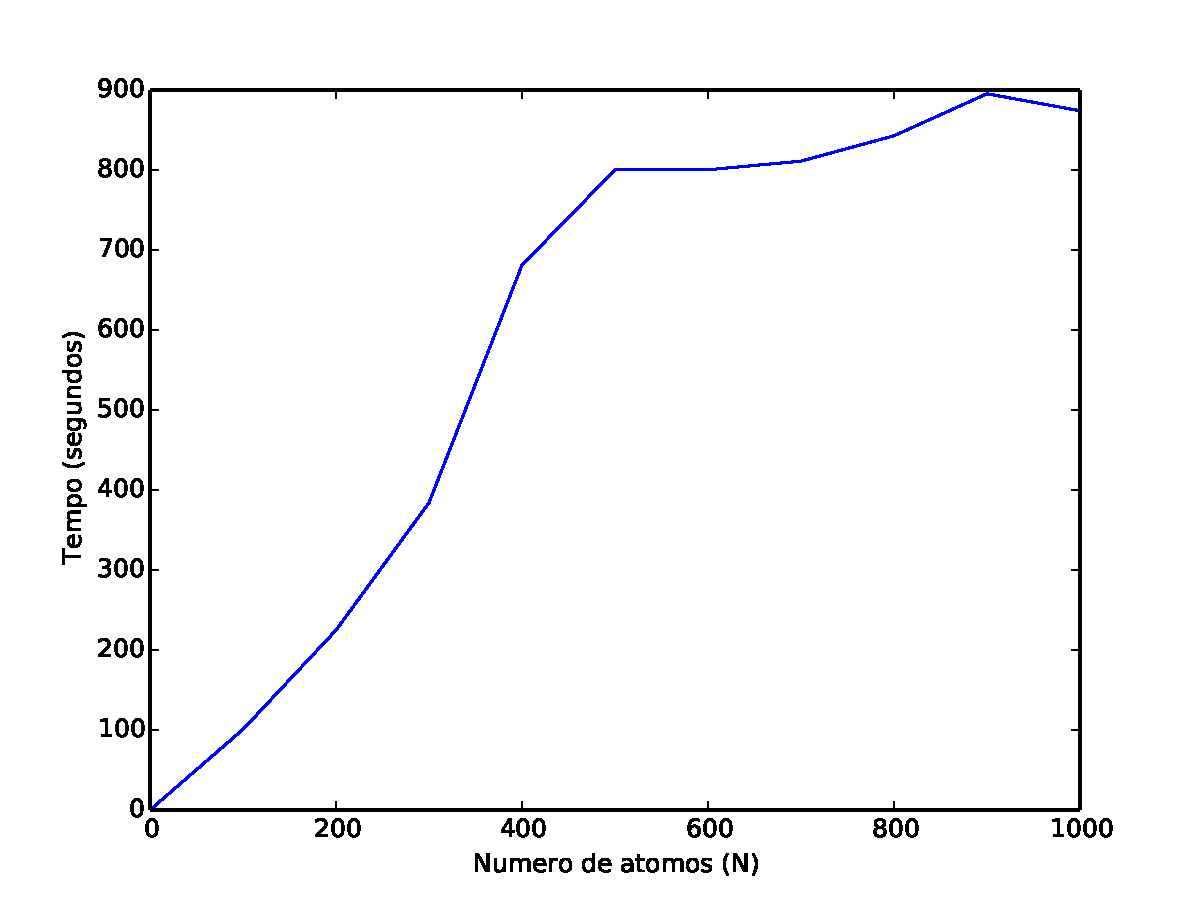
\includegraphics[height=10cm]{images/max3sat_mn80}
			\caption{Curva de resposta de tempo para $M/N=8.0$}
			\label{fig:max3satmn80}
		\end{figure}

\subsection{Experimento 4}
	\subsubsection{Descrição}
		Apresentar 5 gráficos mostrando o tempo de execução em função de $N$ para $K = 2$. Em cada gráfico, o valor de $M / N$ deve ser fixo. Os cinco gráficos devem ser feitos para $N$ variando de 100 a 1000, em intervalos de 100. Os valores de $M / N$ de cada um dos 5 gráficos são 1; 3; 4,3; 6; e 8. Discutir a natureza da curva obtida em cada caso, se polinomial ou exponencial.
	
	\subsubsection{Resultados}
		\begin{table}[!htb]
			\centering{
				\resizebox{.9\columnwidth}{!}{
					\begin{tabular}{|c|r|r|r|r|r|} \hline
						\multicolumn{1}{|c|}{{N}} & \multicolumn{1}{|c|}{{$M/N=1.0$}} & \multicolumn{1}{|c|}{{$M/N=3.0$}} & \multicolumn{1}{|c|}{{$M/N=4.3$}} & \multicolumn{1}{|c|}{{$M/N=6.0$}} & \multicolumn{1}{|c|}{{$M/N=8.0$}} \\ \cline{1-6}
						100    & 0.040 & 0.259 & 0.057  & 0.063 & 0.075 \\\hline
						200    & 0.048 & 18.241 & 0.078  & 0.099 & 0.136 \\\hline
						300    & 0.052 & 0.076 & 0.111 & 0.152 & 0.218 \\\hline
						400    & 0.062 & 0.128 & 0.159 & 0.221 & 0.354 \\\hline
						500    & 0.060 & 0.115 & 0.193 & 0.337 & 0.615 \\\hline
						600    & 0.076 & 0.188 & 0.310 & 0.446 & 0.700 \\\hline
						700    & 0.073 & 0.191 & 0.382 & 0.659 & 0.982 \\\hline
						800    & 0.073 & 0.217 & 0.398 & 0.890  & 1.184 \\\hline
						900    & 0.0790 & 0.272 & 0.551 & 1.128 & 2.731 \\\hline
						1000  & 0.286 & 0.359 & 0.582 & 1.535 & 2.275 \\\hline
					\end{tabular}
        				}
			}
			\label{tab:2satTempos}
			\caption{Comparação de tempos (segundos) de Max 2-SAT}
		\end{table}
		
		\begin{figure}[H]
			\centering
			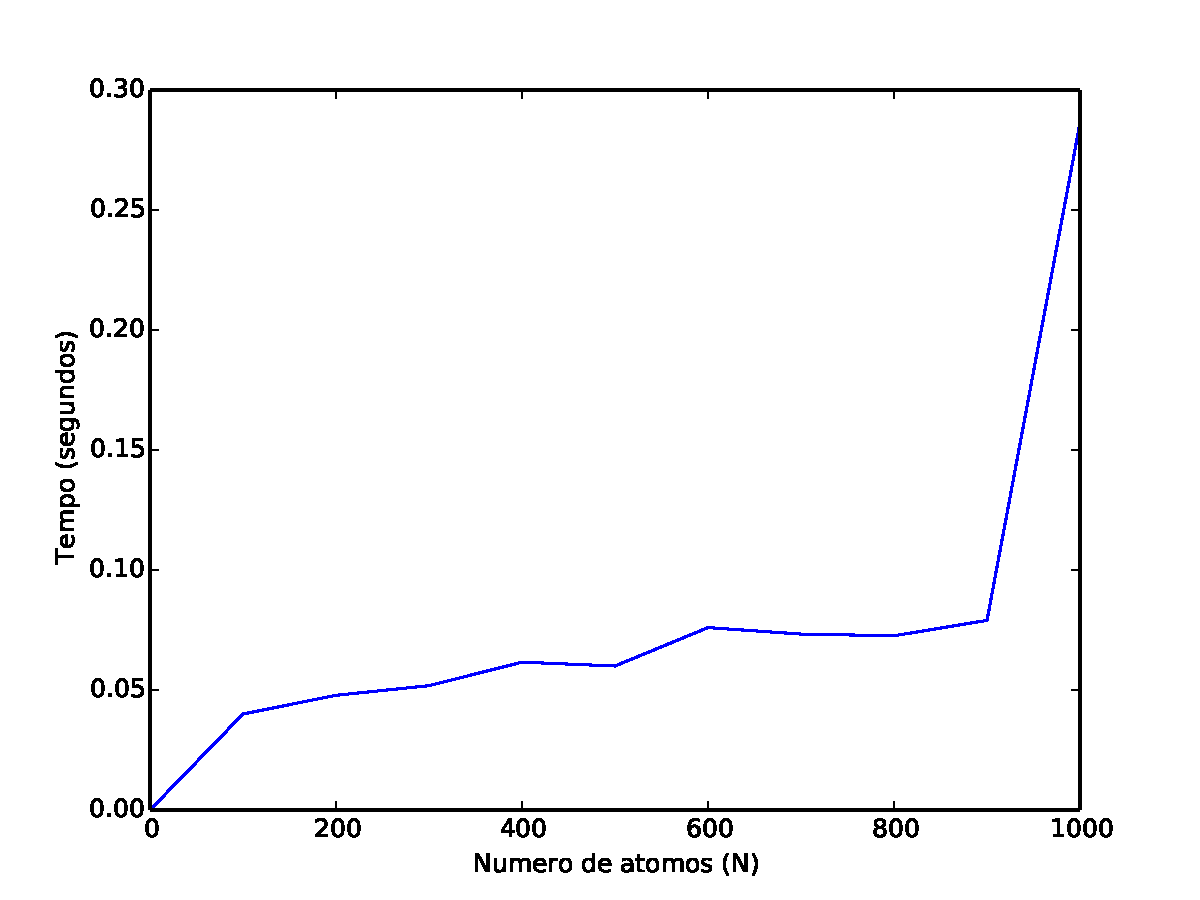
\includegraphics[height=10cm]{images/max2sat_mn10}
			\caption{Curva de resposta de tempo para $M/N=1.0$}
			\label{fig:max2satmn10}
		\end{figure}
		
		\begin{figure}[H]
			\centering
			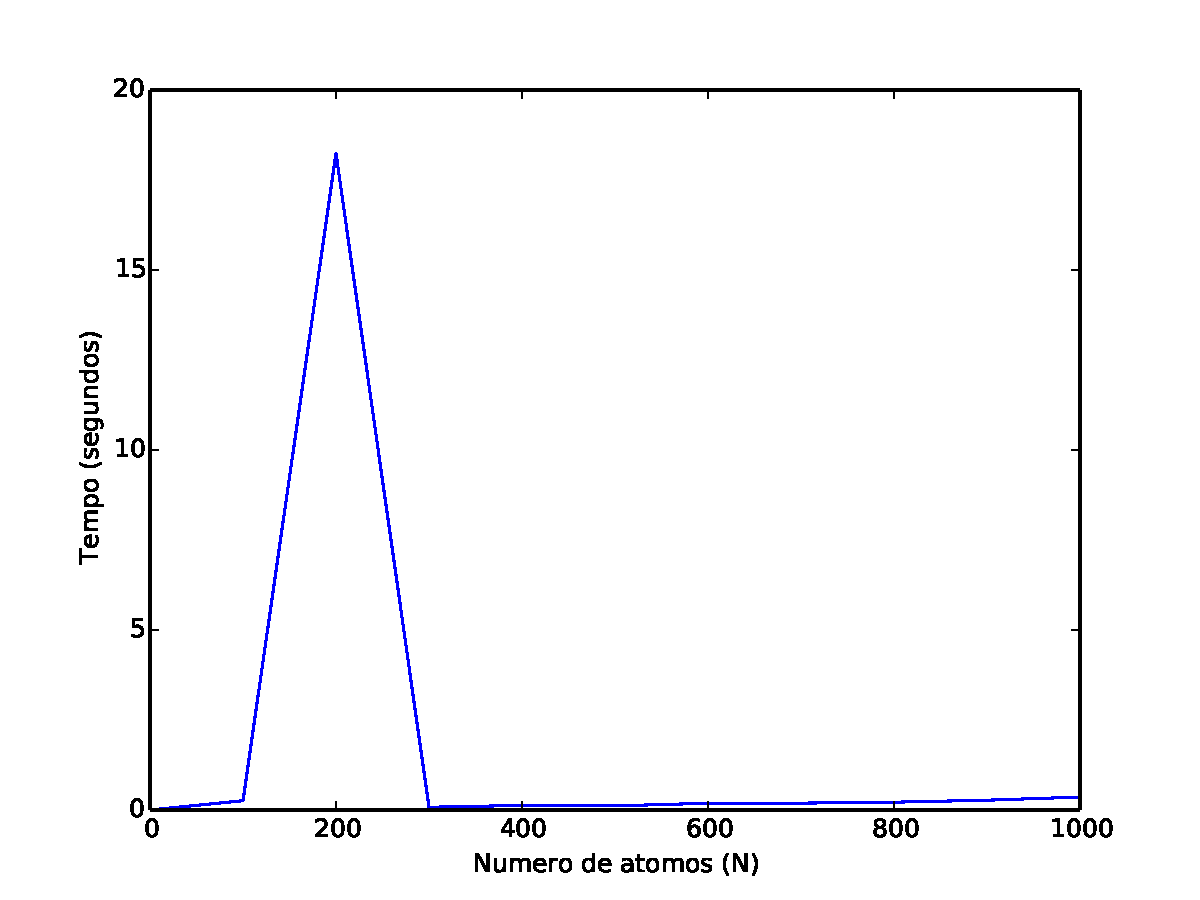
\includegraphics[height=10cm]{images/max2sat_mn30}
			\caption{Curva de resposta de tempo para $M/N=3.0$}
			\label{fig:max2satmn30}
		\end{figure}
		
		\begin{figure}[H]
			\centering
			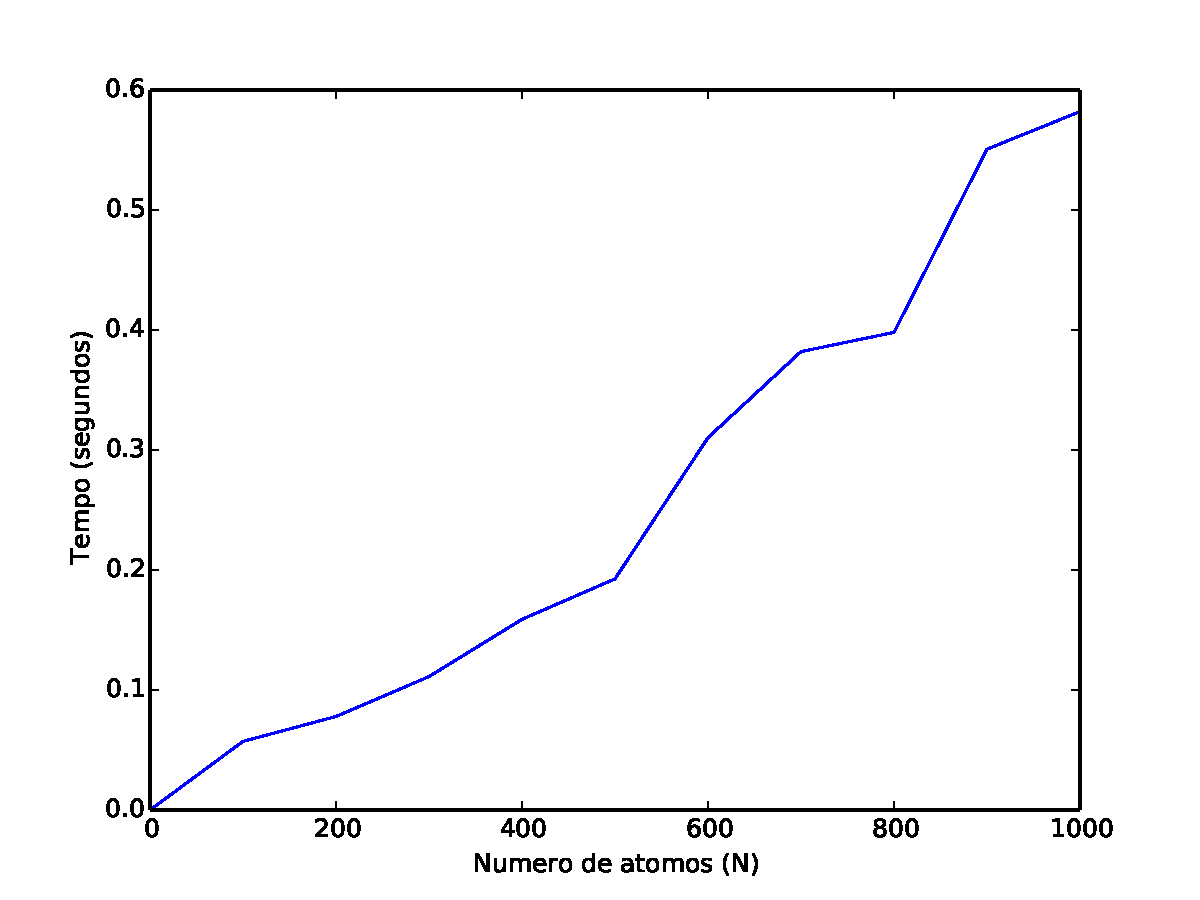
\includegraphics[height=10cm]{images/max2sat_mn43}
			\caption{Curva de resposta de tempo para $M/N=4.3$}
			\label{fig:max2satmn43}
		\end{figure}
		
		\begin{figure}[H]
			\centering
			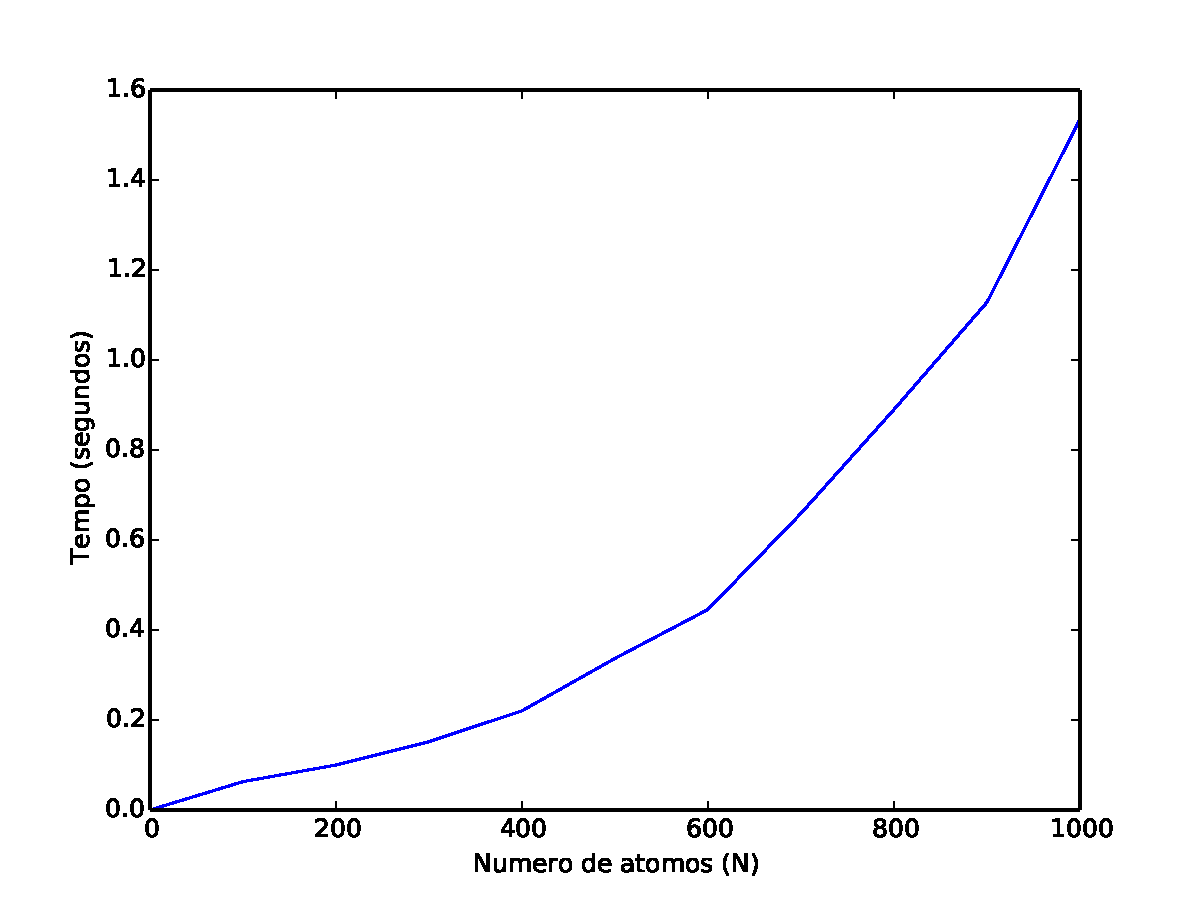
\includegraphics[height=10cm]{images/max2sat_mn60}
			\caption{Curva de resposta de tempo para $M/N=6.0$}
			\label{fig:max2satmn60}
		\end{figure}
		Texto figura 4
		
		\begin{figure}[H]
			\centering
			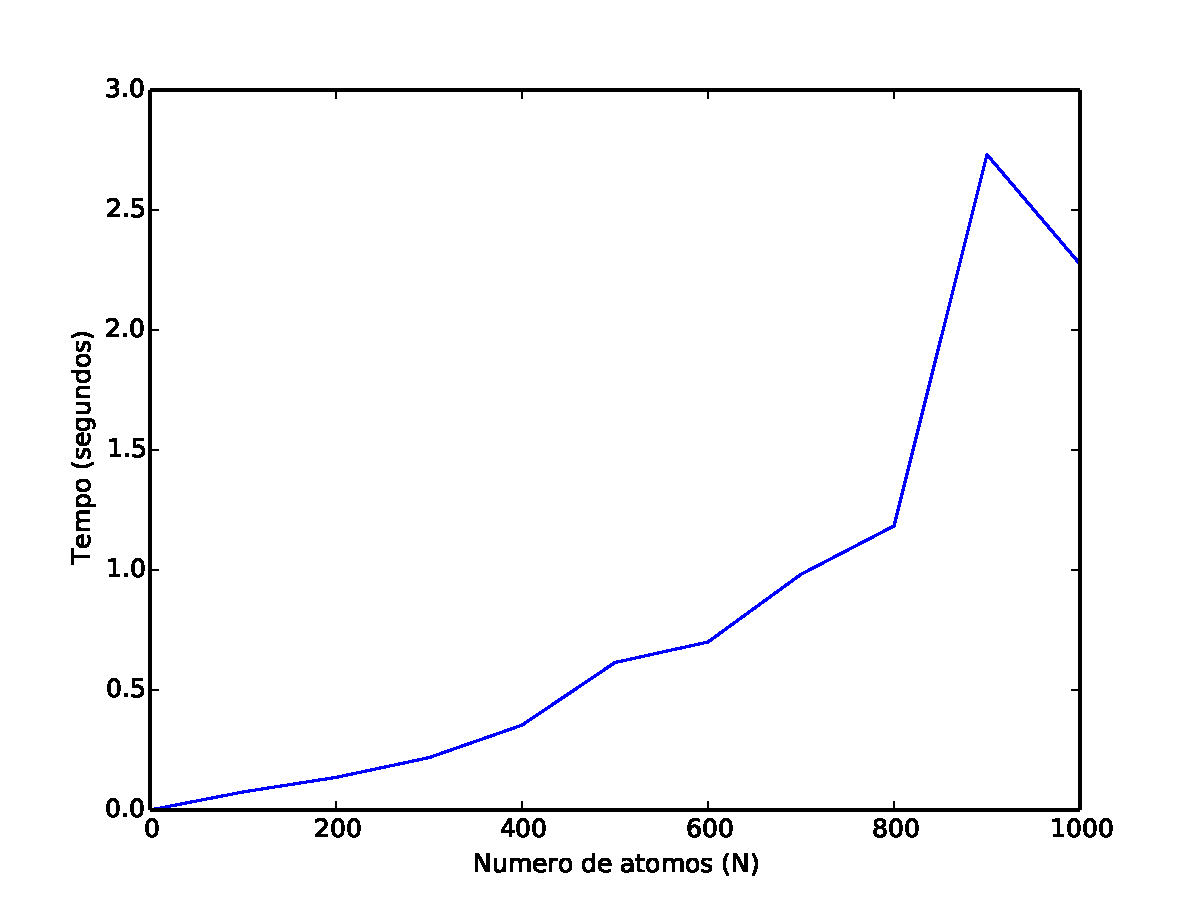
\includegraphics[height=10cm]{images/max2sat_mn80}
			\caption{Curva de resposta de tempo para $M/N=8.0$}
			\label{fig:max2satmn80}
		\end{figure}
		Colocar texto aqui :)
\clearpage 
